% One step of the higher-order tensor renormalisation group, along one
% direction.
%
% Two tensors T of a two-dimensional network are contracted side by side, and
% the two indices that point up -- and the two that point down -- are fused
% into one by an isometry U from a higher-order SVD of the pair, truncated to
% the bond dimension kept. U-dagger closes the other side. What is left has
% one index in each direction again: the coarse-grained tensor T', one site of
% a lattice half as long in this direction. The next step does the other
% direction.
\documentclass[border=4pt]{standalone}
\usepackage{amsmath,amssymb}
\usepackage{tikz-tensors}
\input{notation}
\begin{document}
\begin{tikzpicture}
  \tnstack{H}{2}{top, mid, bot}
  \tnlayer{H}{top}{iso/$U$/2}
  \tnlayer{H}{mid}{coef/$T$, coef/$T$}
  \tnlayer{H}{bot}{isodown/$U^{\dagger}$/2}
  \tnconnect[apart={top, bot}]{H}
  \tnopen{up}{H-top-1}
  \tnopen{down}{H-bot-1}
  \tnopen{left}{H-mid-1}
  \tnopen{right}{H-mid-2}
  \tneq
  \tnstack{K}{1}{top, mid, bot}
  \tnlayer{K}{mid}{coef/$T'$}
  \tnopen{up}{K-mid-1}
  \tnopen{down}{K-mid-1}
  \tnopen{left}{K-mid-1}
  \tnopen{right}{K-mid-1}
\end{tikzpicture}
\end{document}
